% --
% spectrogram

\section{Spectral Features}\label{sec:signal_spec}
Spectral Features, such as a spectrogram, are the most intuitive form to represent audio waveforms. 
They illustrate which frequencies are active at each time instance using a fixed analytic window $t_N$, shifted on the time axis with a time interval, denoted as hop time $t_{hop}$.
The analytic window containing a number of $N$ audio samples, is transformed with the Discrete Time Fourier Transform (DTFT):

% DTFT
\begin{equation}\label{eq:signal_spec_dtft}
    X[k] = \sum_{n=0}^{N-1} x[n] \, e^{-j\frac{2 \pi n}{N}k}
\end{equation}
into the frequency space with frequency index $k$, sample index $n$ and therefore discrete audio samples $x[n]$.
The length of the analytic window in samples $N$ is crucial for the frequency resolution and the lowest frequency that can be represented.
For example, the periodic time of a sound with $f=\SI{20}{\hertz}$ is $t=\frac{1}{f} = \SI{50}{\milli\second}$.
To represent a waveform it would be good to have at least a quarter of its wavelength captured.
Within this thesis, the length of the analytic window is selected to \SI{25}{\milli\second}.

The other important parameter is the hop size (in samples) or hop time, by which the analytical window is shifted on the time axis.
This parameter indicates the resolution in time
In applications like speech processing, the hop time should be selected so that the fastest pronounced phone is within this time span and that changes to other phones are as well captured with enough resolution.
Usually a hop time of $t_{hop}=\SI{10}{\milli\second}$ is chosen (also used within this thesis), but could be also extended like in \cite{Peter2020} to $t_{hop}=\SI{20}{\milli\second}$ for saving computations.




% stft params
% --
% stft params
\begin{table}[ht!]
\begin{center}
\caption{Parameters used for the STFT computation.}
\begin{tabular}{ M{4cm}  M{4cm}}
\toprule
\textbf{Parameter} & \textbf{Value} \\
\midrule
Sampling Frequency & \SI{16}{\kilo\hertz}\\
Analytic window size & \SI{25}{\milli\second}\\
Hop size & \SI{10}{\milli\second}\\
Window Function & Hanning\\
\bottomrule
\label{tab:signal_spec_stft}
\end{tabular}
\end{center}
\end{table}
\FloatBarrier
\noindent



A spectrogram with linear representation is shown in \rfig{spec-lin}.

\begin{figure}[!ht]
  \centering
    \subfigure[left]{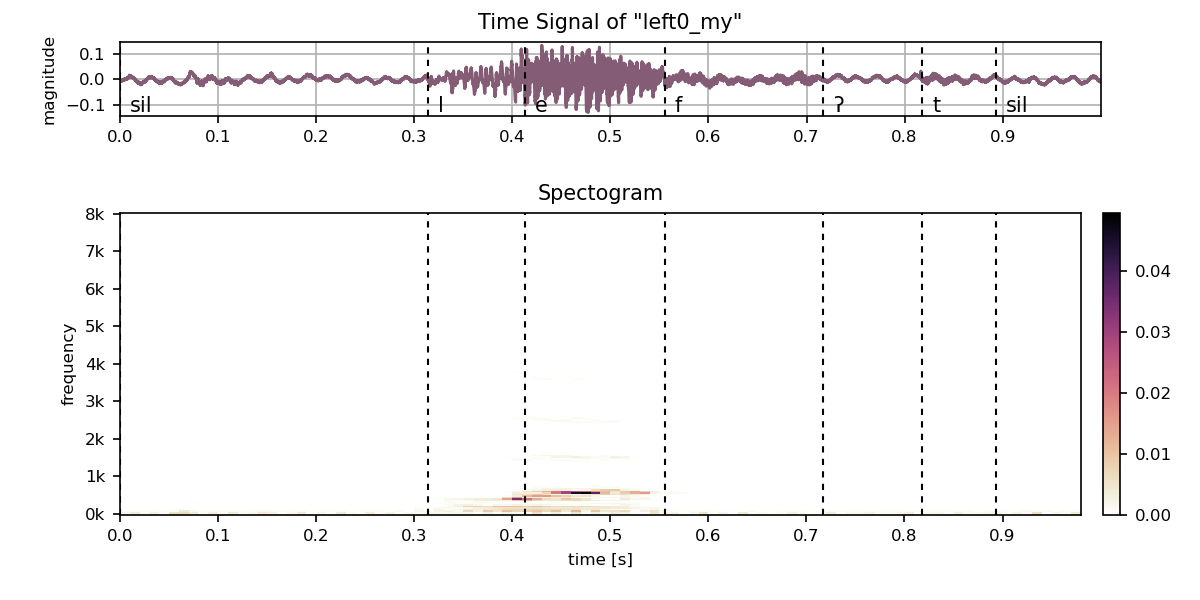
\includegraphics[width=0.45\textwidth]{./3_signal/figs/signal_spec-lin_left0_my}}
    \subfigure[right]{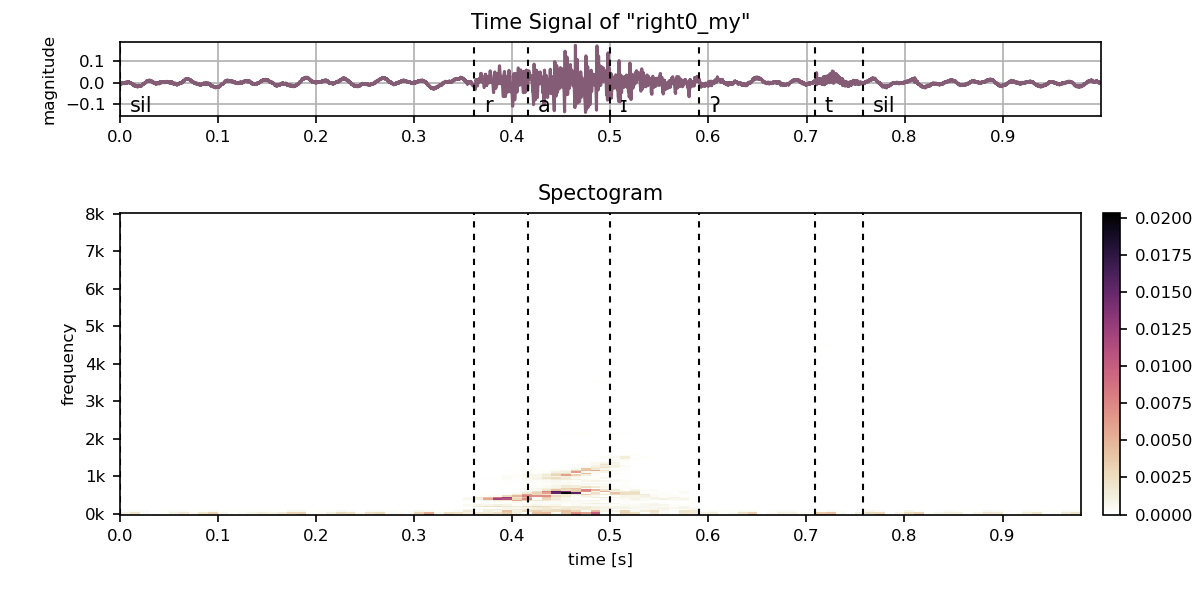
\includegraphics[width=0.45\textwidth]{./3_signal/figs/signal_spec-lin_right0_my}}
    \subfigure[up]{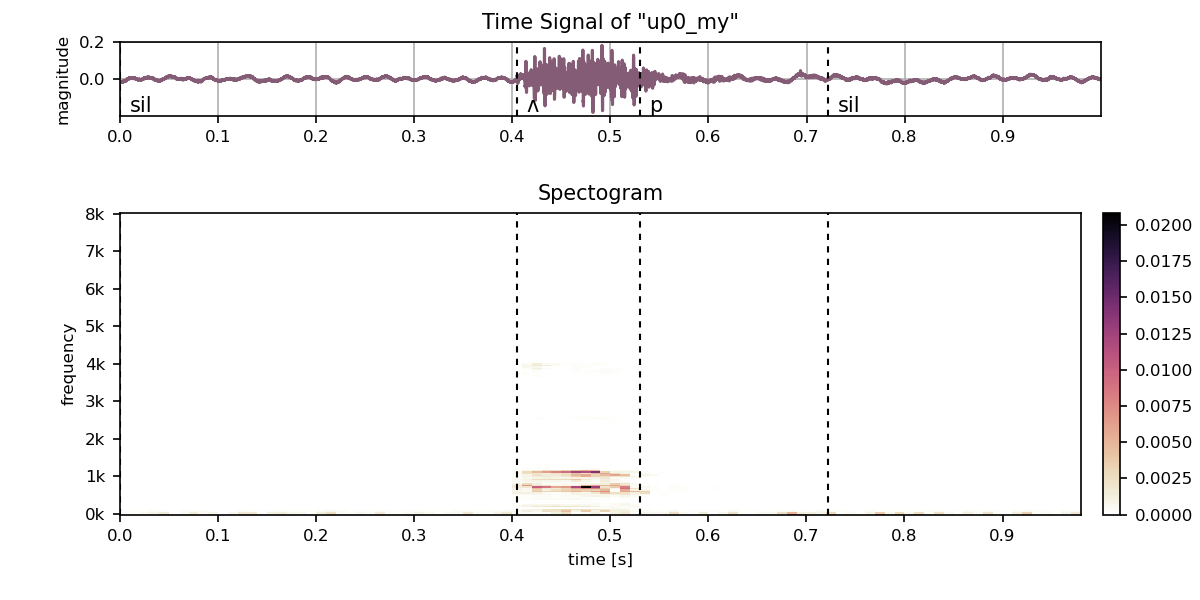
\includegraphics[width=0.45\textwidth]{./3_signal/figs/signal_spec-lin_up0_my}}
    \subfigure[down]{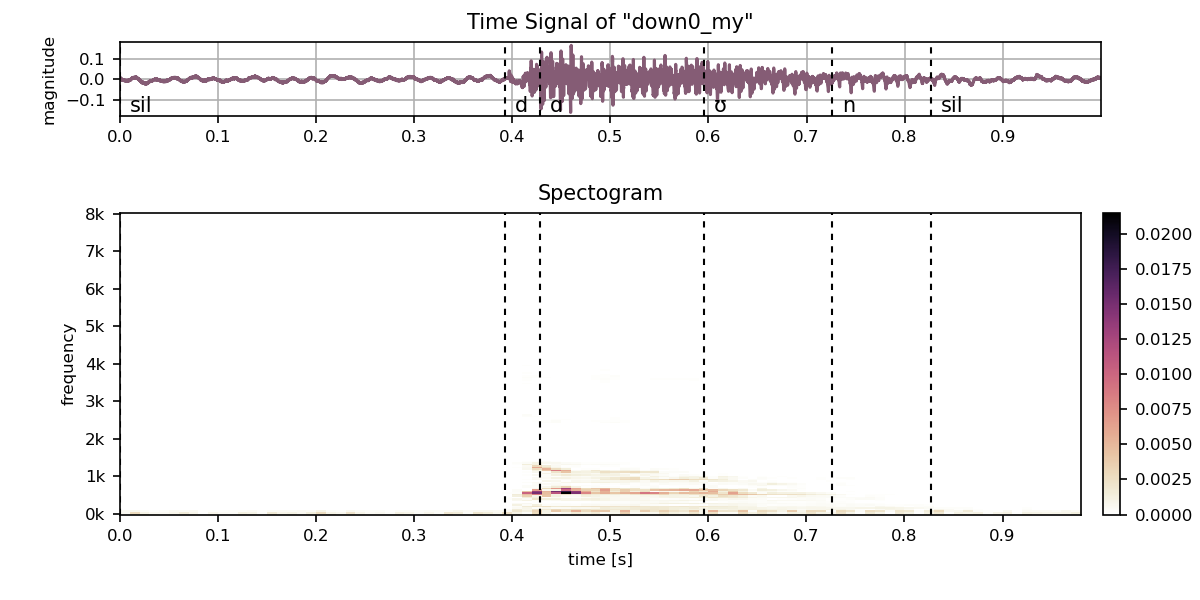
\includegraphics[width=0.45\textwidth]{./3_signal/figs/signal_spec-lin_down0_my}}
    \subfigure[go]{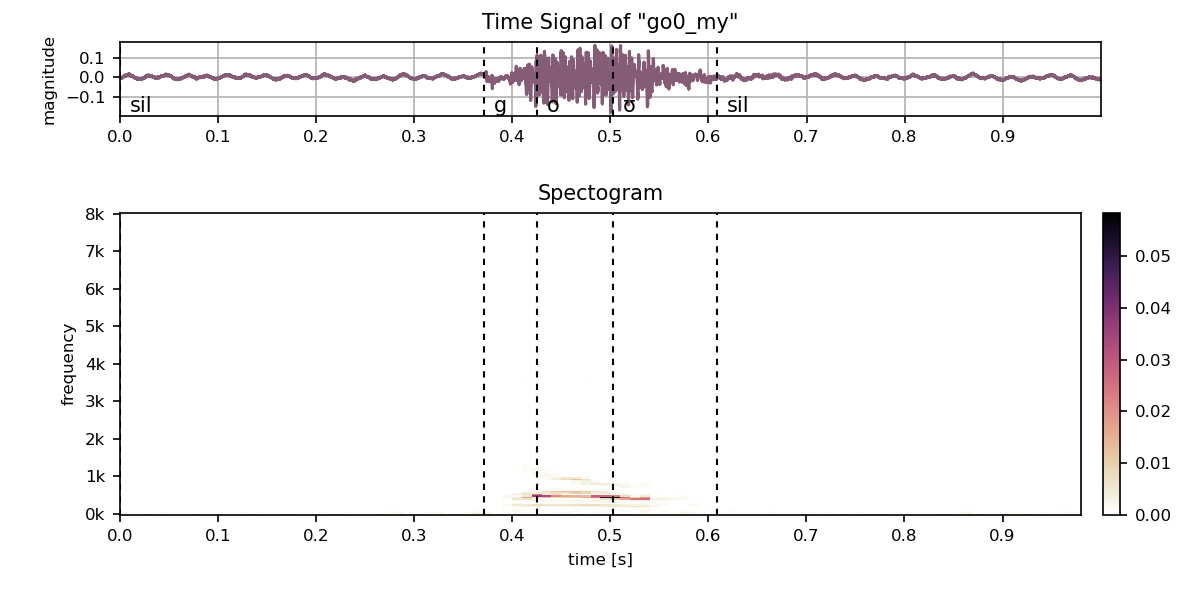
\includegraphics[width=0.45\textwidth]{./3_signal/figs/signal_spec-lin_go0_my}}
  \caption{Spectrogram linear scaled.}
  \label{fig:spec-lin}
\end{figure}
\FloatBarrier
\noindent

One can see here, that most of the energy of the signal is in the lower frequency regions under 1kHz.
It is more interesting to go into the log scale, shown in \rfig{spec-log}

\begin{figure}[!ht]
  \centering
    \subfigure[left]{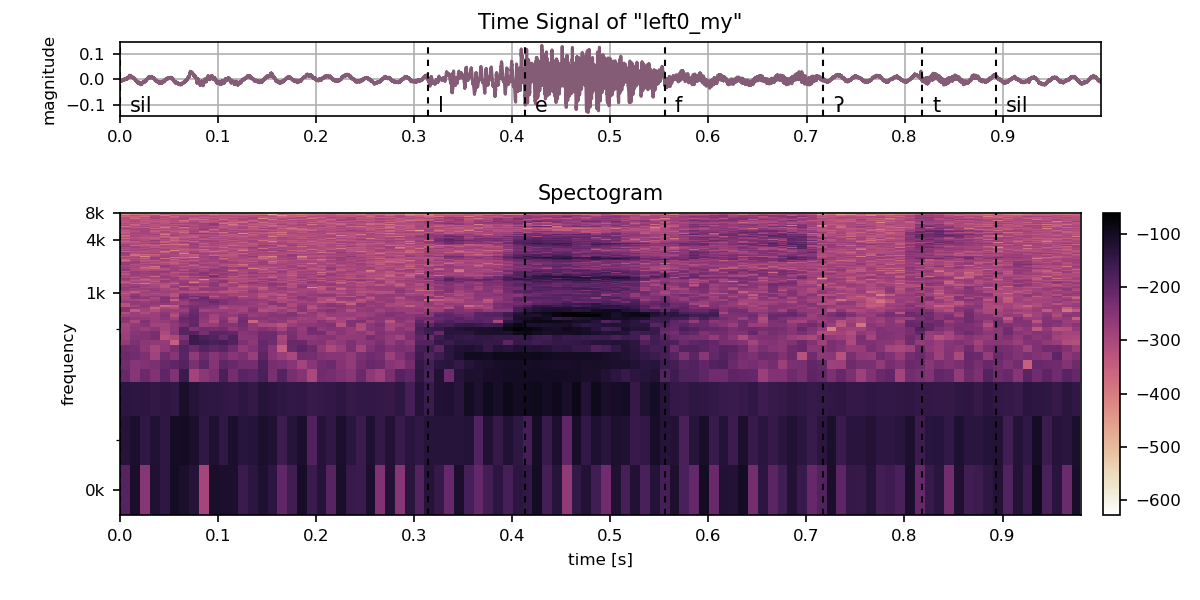
\includegraphics[width=0.45\textwidth]{./3_signal/figs/signal_spec-log_left0_my}}
    \subfigure[right]{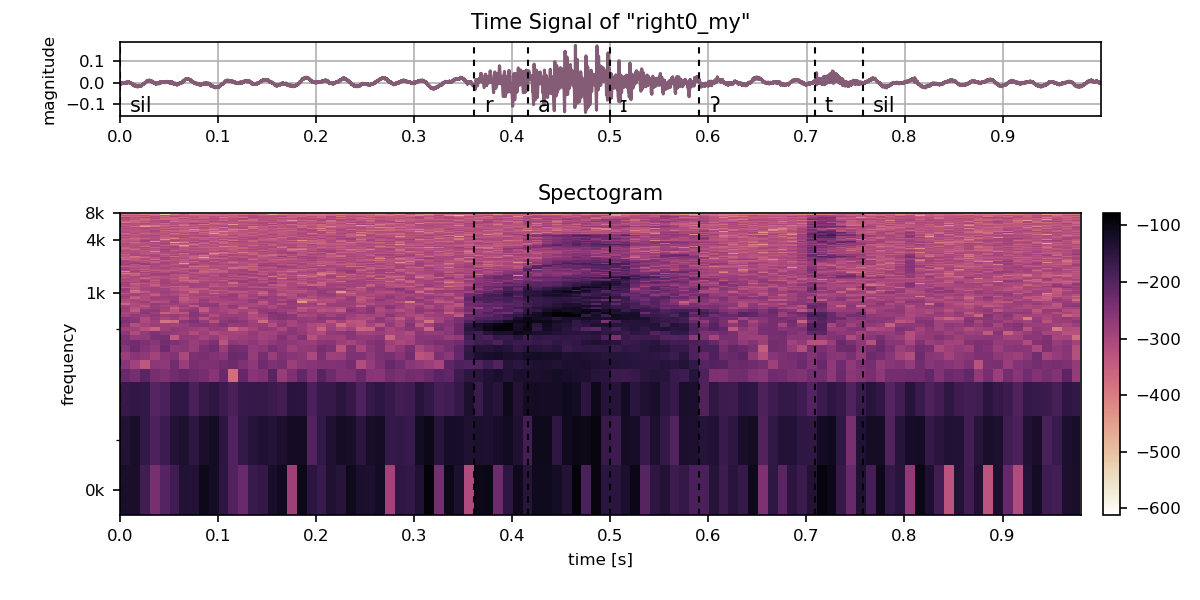
\includegraphics[width=0.45\textwidth]{./3_signal/figs/signal_spec-log_right0_my}}
    \subfigure[up]{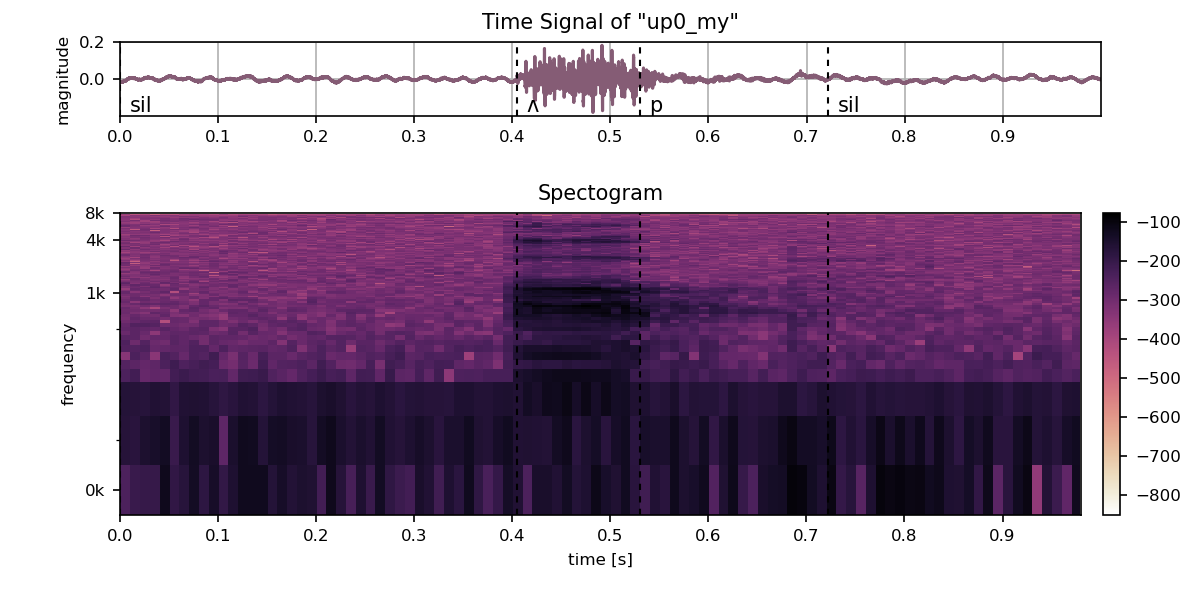
\includegraphics[width=0.45\textwidth]{./3_signal/figs/signal_spec-log_up0_my}}
    \subfigure[down]{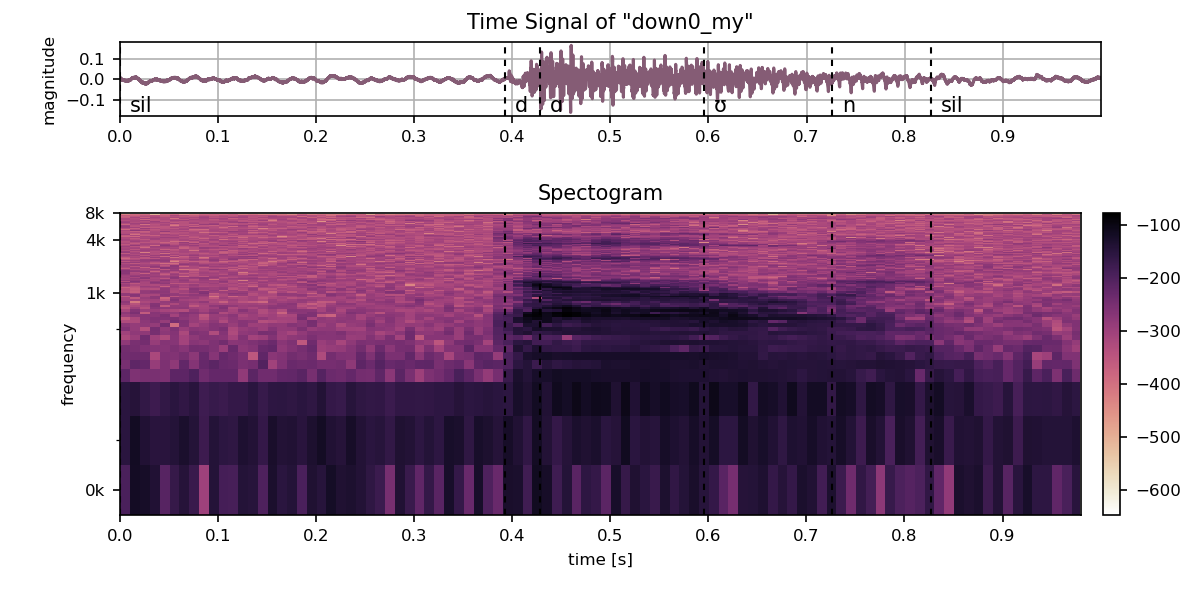
\includegraphics[width=0.45\textwidth]{./3_signal/figs/signal_spec-log_down0_my}}
    \subfigure[go]{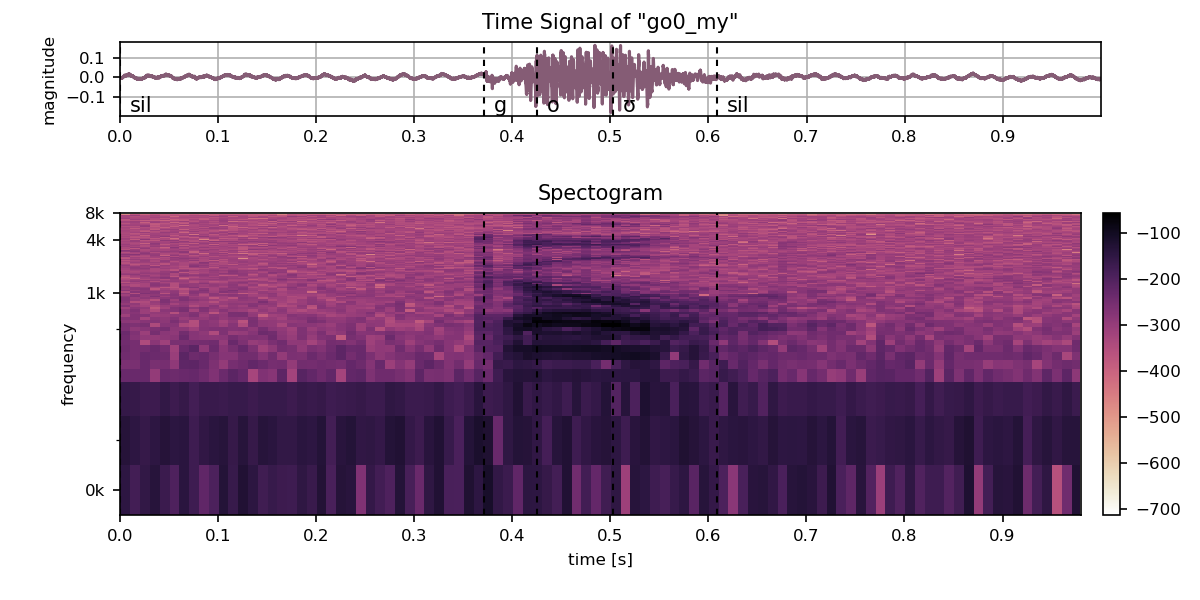
\includegraphics[width=0.45\textwidth]{./3_signal/figs/signal_spec-log_go0_my}}
  \caption{Spectrogram logarithmic scaled.}
  \label{fig:spec-log}
\end{figure}
\FloatBarrier
\noindent